% Geometry, font
\documentclass[12pt, letter]{article}
\usepackage[margin=0.8in]{geometry}
\usepackage[T1]{fontenc}
\usepackage{fourier}
\usepackage{titling}
\setlength{\droptitle}{-5em} 
\usepackage[parfill]{parskip}
\usepackage{graphicx}
\graphicspath{{imgs/}}
\usepackage{hyperref}

% Math stuff
\usepackage{amssymb}
\usepackage{bm}

% Code Highlighting
\usepackage{minted}
\usemintedstyle{solarizedlight}

\author{Zach Neveu}
\title{ Day 9 Notes }

\begin{document}
\maketitle

\section{Agenda}%
\label{sec:agenda}
\begin{itemize}
	\item Quizzes back
	\item No simple mapping from \# to grade - based on "expected number"
	\item Intro to LP
	\item Examples of LP
\end{itemize}

\section{HW \#2}%
\label{sec:hw_#2}
\begin{itemize}
	\item Definition of NP: \textbf{yes} example has certificate which can be verified in polynomial time.
	\item Definition is not symmetrical! 
	\item Many problems in NP have inverse outside of NP
\end{itemize}

\section{Linear Programming}%
\label{sec:linear_programming}
\begin{itemize}
	\item Example: Political Election categories (see day 8)
	\item Ex. Input: \$20k on roads, \$0 on guns, \$4k on farms, \$9k on gas
	\item Minimize $x_1 + x_2 + x_3 + x_4$ (total cost)
\end{itemize}

\begin{center}
\begin{gather*}
20(-2)+0(5)+4(0)+9(10) = 50,000 \\
20(5)+0(2)+4(0)+9(0) = 100,000 \\
20(3)+0(-5)+4(0)+9(-2) = 200,000 \\
\end{gather*}
\end{center}

\subsection*{General Linear Program}
Given a set of constants $a_1, \ldots, a_n$ and a set of variables $x_1, \ldots, x_n$, a \textbf{linear function} $f$ on the variables is:
\[
f(x_1,\ldots,x_n) = a_1(x_1)+\ldots+a_n(x_n) = \sum_{\alpha=1}^{n} a_{\alpha}x_{\alpha}
\] 
Given a constant $b$ and a linear function $f$, \\
$f\left( \right) \le b$ and $f\left( \right) \ge b$ are linear inequalities \\
$f\left( \right) = b$ is a linear equality \\
$<$ and $>$ are not linear! \\

\textbf{LP Problem: } The problem of maximizing or minimizing a linear function subject to a finite set of linear constraints. \\
Example: \\
Maximize: $x_1 + x_2$ \\
Subject to: \\
\begin{gather*}
4x_1-x_2 \le 8 \\
2x_1+x_2 \le 10 \\
5x_1-2x_2 \ge -2 \\
x_1,x_2 \ge 0 \\
\end{gather*}

\begin{figure}[h]
	\centering
	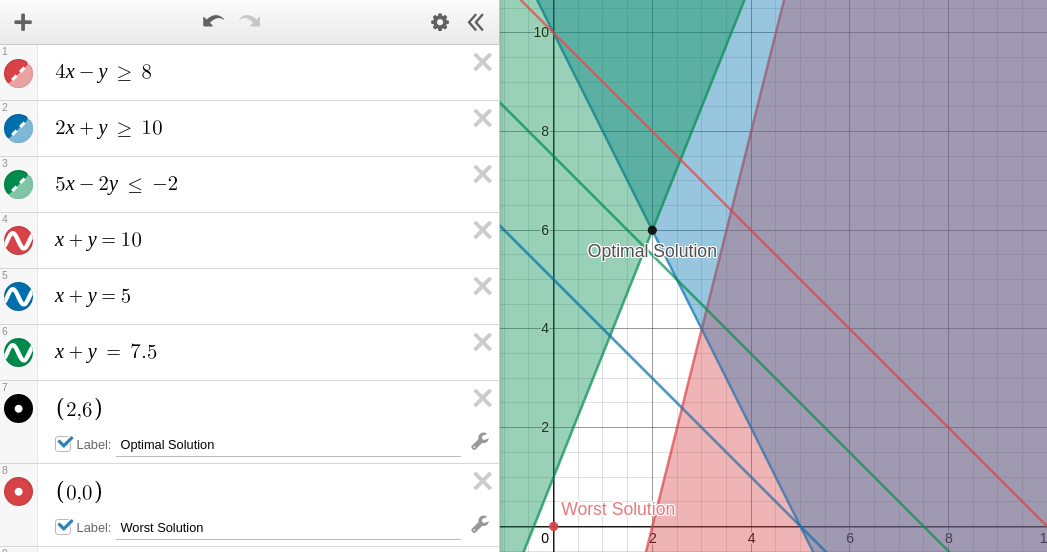
\includegraphics[width=0.8\textwidth]{graph2}
	\caption{Graph of Solution Space: where all regions overlap is valid (marked in white). $x=y$ lines show value -> further from origin is better.}
	\label{fig:graph}
\end{figure}

\subsection*{Example: Reclaiming Solid Waste}
Inputs are 3 types of materials: 1,2\&3 \\
\begin{table}[h]
	\centering
	\caption{Material Availability}
	\begin{tabular}{cc}
	Material & Available Pounds/Week \\
	\hline
	1 & 100 \\
	\hline
	2 & 200 \\
	\hline
	3 & 300 \\
	\hline
	\end{tabular}
\end{table}

\begin{table}[h]
	\centering
	\caption{Grades}
	\label{tab:label}
	\begin{tabular}{ccc}
	\hline
	Grade & Spec & profit/pound \\
	\hline
	A & $M_1 \le 30\%, M_2 \le 40\%$ & 5 \\
	\hline
	B & $M_2 = 50\%, M_2 \le 20\%$ & 10 \\
	\hline
	\end{tabular}
\end{table}

Problem: \\
Maximize: $5Y_A+10Y_B$ \\
Let: $Z_{MN} = $ the proportion of grade $M$ that is material $N$ \\
Subject to: \\
\begin{gather*}
Z_{A_1} \le 0.3 \\
Z_{A_2} \le 0.4 \\
Z_{B_2} = 0.5 \\
Z_{B_3} \le 0.2 \\
Y_A * Z_{A_1} + Y_B * Z_{B_1} \le 100 \\
\vdots \\
\end{gather*}
UH OH! This multiplies variables which isn't linear\ldots \\
Fix: \\
Let: $X_{MN} =$ \underline{amount} of Material $N$ in grade  $M$ \\
New Constraints: \\
\begin{gather*}
X_{A_1}+X_{B_1} \le 100 \\
X_{A_2}+X_{B_2} \le 200 \\
X_{A_3} + X_{B_3} \le 300 \\
\end{gather*}
New Objective Function: \\
Maximize: $5(X_{A_1}+X_{A_2}+X_{A_3})+10(X_{B_1}+X_{B_2}+X_{B_3})$

\subsection*{Takeaways}
\begin{itemize}
	\item Variable choices matter! Effects speed and solve-ability
	\item Seemingly non-linear variables can be re-written as linear variables
\end{itemize}

\subsection*{Standard Form}
Given constants $c_1,\ldots,c_n$, $b_1,\ldots,b_m$ and $m*n$ values $a_g$ for $i=1\rightarrow m$ and $j=1\rightarrow n$, find $x_1,\ldots,x_n$ such that: \\
Maximize: $ \sum_{j=1}^{n} c_j x_j$ \\
Subject to: $ \sum_{i=1}^{n} a_{ij}x_j \le b_i$ for $i=1 \rightarrow m$ \\
 $x_j \ge 0$ for $j=1\rightarrow n$ \\
$n=$ \# variables
$m=$ \# constraints

\begin{itemize}
	\item In standard form, all variables $x \ge 0$
	\item Only maximization as operation
	\item 
\end{itemize}

\subsection*{Concise Standard Form}
\begin{itemize}
	\item $\bm{A} = (a_{ij})$
	\item $\bm{b} = (b_i)$ 
	\item $\bm{c} = (c_j)$
	\item $\bm{x} = (x_j)$
\end{itemize}
An LP formulation in standard form is: maximize $C^{T}x$ subject to $Ax \le b$,  $x \ge 0$.
\end{document}
